\documentclass{article}
\usepackage[utf8]{inputenc}
\usepackage[italian]{babel}
\usepackage{amsmath}
\usepackage{amssymb}
\usepackage{siunitx}
\usepackage{tabularray}
\usepackage{graphicx}
\usepackage{float}
\usepackage{minted}
\usepackage[page]{appendix}
\usepackage{mathtools}
\newcommand*{\diam}{\varnothing}
\newcommand*{\best}[1]{{#1}_\text{best}}
\newcommand*{\bestp}[1]{{\left(#1\right)}_\text{best}}
\newcommand*{\pbest}[1]{\left({#1}_\text{best}\right)}
\newcommand*{\pbestp}[1]{\left({\left(#1\right)}_\text{best}\right)}
\newcommand*{\errrel}[1]{\frac{\delta #1}{{#1}_\text{best}}}
\title{
    Laboratorio di Fisica 1\\
    R6: Misura dei calori specifici di materiali ignoti
}
\author{Gruppo 17: Bergamaschi Riccardo, Graiani Elia, Moglia Simone}
\date{6/12/2023 – 13/12/2023}
\makeindex
\begin{document}

\maketitle

\begin{abstract}
    Il gruppo di lavoro ha misurato il calore specifico di tre solidi distinti
    per risalirne alla natura; a questo fine, è stato necessario determinare
    le caratteristiche termiche del calorimetro
    (capacità termica e conducibilità).
\end{abstract}

\setcounter{section}{-1}
\section{Materiali e strumenti di misura utilizzati}
\begin{center}
    \begin{tblr}{ |Q[l,m]|Q[c,m]|Q[c,m]|Q[c,m]| }
        \hline
        \textbf{Strumento di misura} & \textbf{\:\:\:\:\:Soglia\:\:\:\:\:} & \textbf{Portata} & \textbf{Sensibilità} \\
        \hline
        Termometro digitale & $\qty{0.1}{\degree C}$ & N./A. & $\qty{0.1}{\degree C}$ \\
        \hline[dashed]
        Cronometro & $\qty{0.5}{s}$ & N./A. & $\qty{0.5}{s}$ \\
        % \hline[dashed]
        % Termometro a mercurio & $\qty{0.1}{\degree C}?$ & $\qty{100}{\degree C}?$ & $\qty{0.1}{\degree C}?$ \\
        \hline[dashed]
        Barometro & $\qty{1}{hPa}?$ & $\qty{14000}{hPa}$ & $\qty{1}{hPa}$ \\
        \hline[dashed]
        Cilindro graduato & $\qty{1}{mL}$ & $\qty{100}{mL}$ & $\qty{1}{mL}$ \\
        \hline[dashed]
        Bilancia di precisione & $\qty{0.01}{g}$ & $\qty{4100.00}{g}$ & $\qty{0.01}{g}$ \\
        \hline
        \hline
        \textbf{Altro} & \SetCell[c=3]{l} \textbf{Descrizione/Note} \\
        \hline
        Calorimetro & \SetCell[c=3]{l} {Quasi adiabatico.} \\
        \hline[dashed]
        {Fornelletto e pentolino} & \SetCell[c=3]{l} {Per scaldare acqua e campioni.} \\
        \hline[dashed]
        Tre campioni solidi & \SetCell[c=3]{l} {Li chiameremo $A$, $B$ e $C$.} \\
        \hline
    \end{tblr}
\end{center}

\section{Misurazione della massa equivalente}

Il calorimetro, per quanto isolante termicamente, comunque non è completamente
adiabatico. Pertanto, prima di procedere con la misura indiretta dei calori
specifici dei campioni di materiale ignoto, è necessario ottenere una stima
della capacità termica del calorimetro $C_\text{cal}$.

Per semplificare i calcoli, abbiamo definito “massa (d'acqua) equivalente
(in senso termico) al calorimetro” come la quantità:
\[m_\text{eq} \coloneqq \frac{C_\text{cal}}{c_{\text{H}_2\text{O}}}\]

\emph{
\textbf{Osservazione.} La massa equivalente ci dà anche un'idea di
quanto il calorimetro disturbi le misure.
}

\subsection{Esperienza e procedimento di misura}

\begin{enumerate}
    \item
        Misuriamo, mediante la bilancia di precisione, la massa del
        calorimetro vuoto (coperchio compreso):
        $m_\text{cal} = \left(781.91\pm0.01\right) \unit{g}$
    \item
        Versiamo, aiutandoci col cilindro graduato, circa $\qty{100}{mL}$
        di acqua distillata ($c_{\text{H}_2\text{O}}=\qty{4186}{J\,kg^{-1}K^{-1}}$)
        a temperatura ambiente $T_\text{amb}$ nel calorimetro.
        Per avere una stima più accurata di questa quantità di acqua,
        misuriamo la massa complessiva del calorimetro dopo questa operazione.
        In questo modo, otteniamo indirettamente la massa d'acqua “fredda”:
        $m_\text{fredda} = \left(99.35\pm0.02\right) \unit{g}$
    \item
        Scaldiamo nel pentolino altri $\qty{100}{mL}$, circa, di acqua distillata,
        fino al punto di ebollizione $T_\text{eb}$.
    \item
        Inserito nel calorimetro il termometro digitale, avviamo l'acquisizione dati
        (a intervalli di $\qty{0.5}{s}$).
        Riapriamo poi il calorimetro e vi versiamo all'interno,
        velocemente, l'acqua calda. Infine, richiudiamo il coperchio.
    \item
        Dopo una decina di minuti, interrompiamo l'acquisizione, estraiamo il
        termometro e misuriamo nuovamente la massa del sistema.
        In questo modo, per differenza, otteniamo la massa dell'acqua calda che
        avevamo versato nel calorimetro\footnote{
        Si noti che questa massa è minore di quella che avevamo versato
        nel pentolino, poiché una parte dell'acqua è evaporata. Misurare la massa
        alla fine dell'esperimento, per differenza, ci permette di non doverne
        tener conto successivamente. Possiamo infatti considerare il calorimetro
        come un sistema chiuso: finché non lo apriamo, la massa complessiva
        non cambia.
        }:
        $m_\text{calda} = \left(85.12\pm0.03\right) \unit{g}$
\end{enumerate}

\emph{
\textbf{Osservazione.} È meglio che i due volumi d'acqua siano molto simili e che
la loro somma sia pressoché pari al volume che utilizzeremo nella seconda parte
dell'esperimento, in modo che il calorimetro si bagni allo stesso modo.
}

\subsection{Analisi dei dati raccolti e conclusioni}
Detta $T_\text{eq}$ la temperatura di equilibrio del sistema, vale:
\[
m_\text{calda} (T_\text{eb} - T_\text{eq}) =
(m_\text{fredda} + m_\text{eq})(T_\text{eq} - T_\text{amb})
\]
da cui:
\[
m_\text{eq} = \frac{T_\text{eb}-T_\text{eq}}{T_\text{eq}-T_\text{amb}} m_\text{calda} - m_\text{fredda}
\]

Di seguito riportiamo, in un grafico, i dati raccolti dal termometro digitale.

\begin{center}
    \begin{figure}[H]
        % trim={< v > ^}
        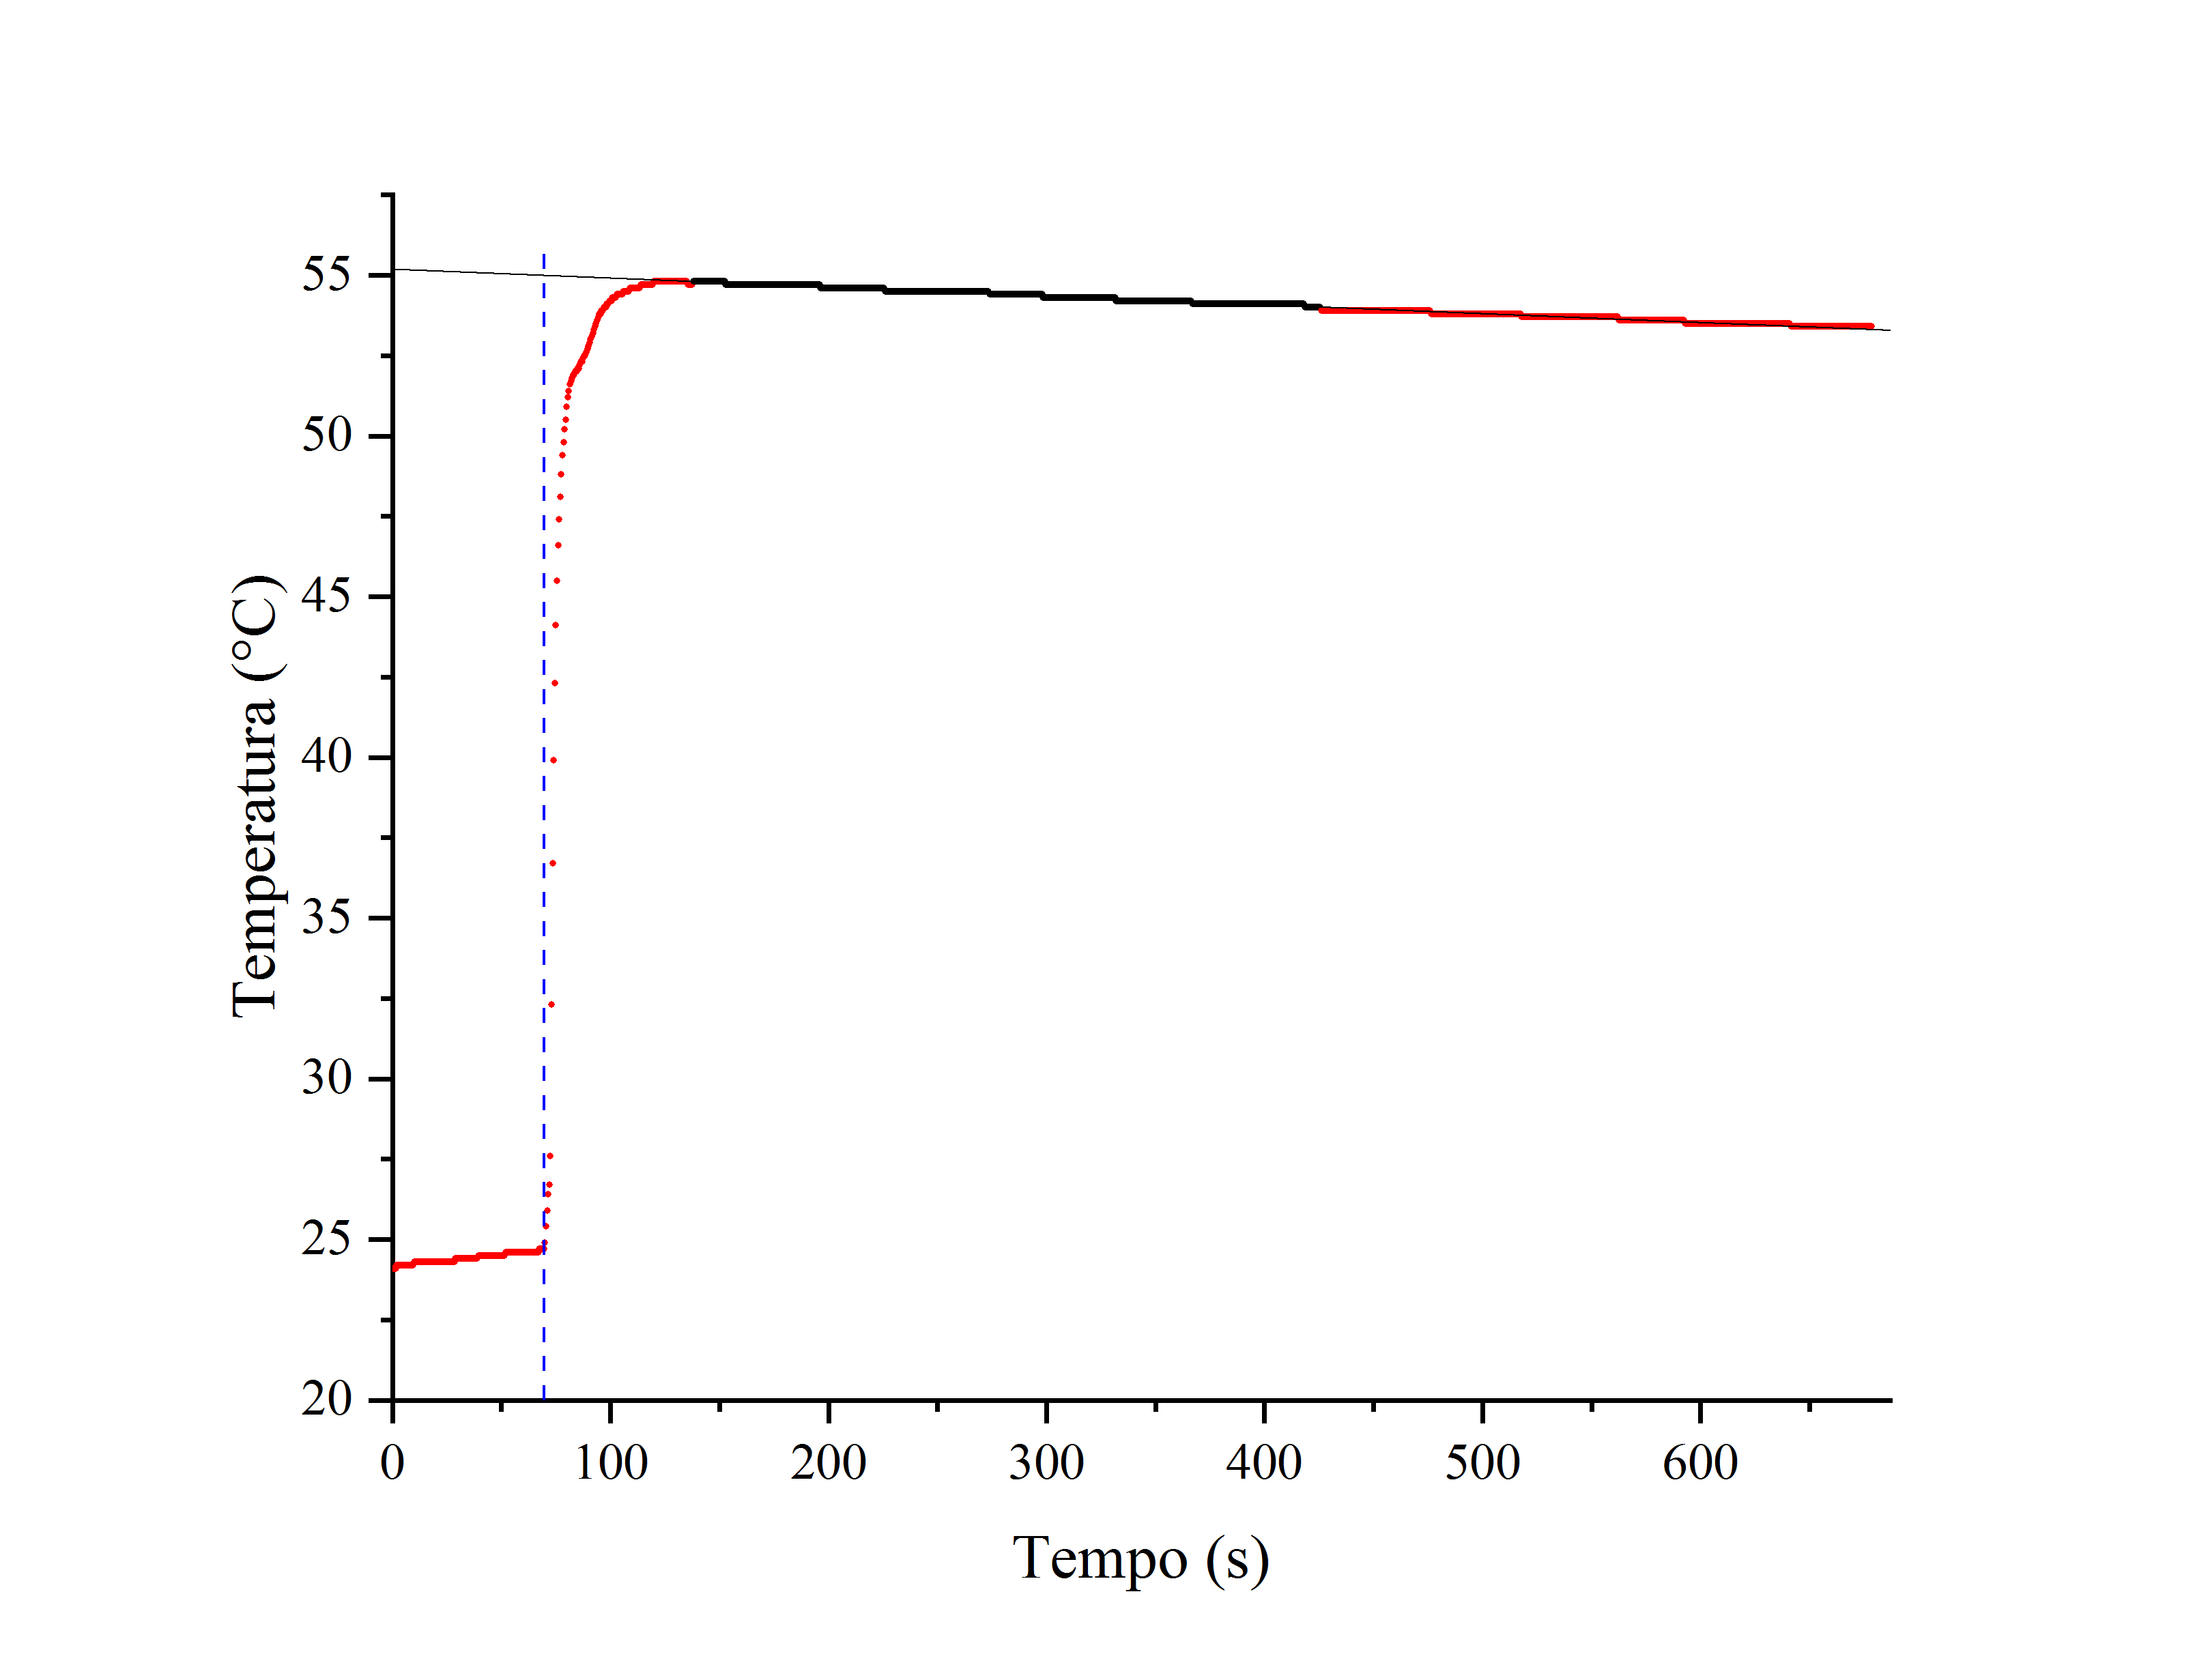
\includegraphics[trim={2cm .5cm 2cm 2.1cm},clip,width=\textwidth]{img/RegH2O.jpg}
        \caption{I dati raccolti col termometro.
        In nero, appena visibile, una retta di regressione sull'intervallo di dati indicato in nero.
        In blu, l'istante di tempo nel quale abbiamo inserito l'acqua calda.
        L'ordinata del punto di intersezione fra le due rette è la temperatura di equilibrio.
    }
    \end{figure}
\end{center}

Eseguendo una regressione lineare sui dati raccolti dal termometro digitale, rappresentati nel    %TODO: spiegare la regressione?
seguente grafico, abbiamo trovato che $T_\text{eq} = \qty{55.0}{\degree C}$. Dunque:    %TODO: mettiamo il grafico?

ovvero $m_\text{equiv} = (24.61116505 \pm 3)\,\unit{g}?$. Ora che abbiamo ottenuto questo valore, possiamo calcolare
i calori specifici dei metalli di cui sono composti i campioni.



\section{Misurazione del calore specifico dei materiali ignoti}

\subsection{Esperienza e procedimento di misura}

\begin{enumerate}
    \item
        Versiamo nel pentolino una quantità d'acqua tale da permettere l'immersione
        completa dei campioni in essa e la scaldiamo. Per fare ciò più velocemente
        e assicurarci di essere in stato di ebollizione, regoliamo la temperatura
        della piastra a $T>\qty{100}{\degree C}$.
    \item
        Misuriamo $\qty{200}{mL}$ di acqua, distillata ed a temperatura ambiente,
        e la versiamo nel calorimetro.
    \item
        Per ogni solido ($A$, $B$ e $C$):
    \begin{enumerate}
        \item
            Ne misuriamo la massa con la bilancia di precisione.
        \item
            Una volta che l'acqua nel pentolino si trova in corrispondenza della
            transizione di fase, lo immergiamo in essa in modo che raggiunga la
            $T$ del sistema.
        \item
            Quando anch'esso raggiunge la temperatura di $\qty{100}{\degree C}$,
            lo spostiamo nel calorimetro e mescoliamo nuovamente. Come prima, sarà
            il termometro digitale a darci il valore di $T$ in funzione del tempo.
    \end{enumerate}
\end{enumerate}



\subsection{Analisi dei dati raccolti e conclusioni}
Grazie alle leggi della termodinamica sappiamo che:
    \[
        m_\text{met} c_\text{met} (T_\text{met}-T_\text{eq}) =
        (c_\text{acqua} m_\text{acqua} + C_\text{calorimetro}) (T_\text{eq}-T_\text{acqua})
    \]
Conoscendo il valore di $m_\text{equiv}$, possiamo scrivere:
    \[
        m_\text{met} c_\text{met} (T_\text{met}-T_\text{eq}) =
        (m_\text{acqua} + m_\text{equiv}) c_\text{acqua} (T_\text{eq}-T_\text{acqua})
    \]

Eseguendo una regressione lineare sui dati raccolti dal termometro digitale, rappresentati nel    %TODO: spiegare la regressione?
seguente grafico, abbiamo trovato calcolato il valore di $T_\text{eq}$ per ogni solido. Dunque:    %TODO: mettiamo i grafici?
    \[
        c_\text{met} = \frac{(m_\text{acqua} + m_\text{equiv}) c_\text{acqua} (T_\text{eq}-T_\text{acqua})}
        {m_\text{met} (T_\text{met}-T_\text{eq})}
    \]

Nella seguente tabella riportiamo i valori ottenuti per ogni solido con le relative incertezze, che abbiamo calcolato con la
propagazione standard degli errori in quanto piccole, sistematiche e indipendenti.

\begin{center}
    \begin{tabular}{ |c|c|c|c| }
        \hline
        \emph{Campione} & $m$ ($\unit{g}$) & $T_\text{eq}$ ($\unit{\degree C}$) & $c$ ($\unit{J \, {kg}^{-1} {K}^{-1} }$) \\
        \hline
        $A$ & $12.43 \pm 0.01$ & $25.2 \pm 0.2$ & $500.9617709 \pm 0$ \\
        $B$ & $28.73 \pm 0.01$ & $25.9 \pm 0.2$ & $345.7664279 \pm 0$ \\    %TODO: calcolare i valori
        $C$ & $44.86 \pm 0.01$ & $26.0 \pm 0.2$ & $110.4618573 \pm 0$ \\
        \hline
    \end{tabular}
\end{center}


\section{Misurazione del tempo caratteristico (del calorimetro?)}

\subsection{Esperienza e procedimento di misura}

\begin{enumerate}
    \item
        Misuriamo $\qty{200}{mL}$ di acqua distillata e la scaldiamo con nel
        pentolino.    %TODO: per quanto? o fino a che temperatura?
    \item
        Nel calorimetro, in partenza vuoto, versiamo l'acqua e la lasciamo
        raffreddare per circa un'ora registrandone la temperatura.
\end{enumerate}

\subsection{Analisi dei dati raccolti e conclusioni}
L'ultima cosa che analizzeremo è la discesa esponenziale della temperatura    %TODO: cambiare la parola "cosa"
dell'acqua dentro al calorimetro. La legge che segue questa discesa è:
\[
    (T-T_\text{amb.})=(T_0-T_\text{amb.}) e^{-t/\tau}
\]

Ne calcoleremo, in particolare, il tempo caratteristico, ovvero la quantità
di tempo $\tau$ che impiega l'acqua all'interno del calorimetro ad abbassare
la sua temperatura di $(T_0 - T_\text{amb})e$ volte.

\emph{
    \textbf{Notazione.} Indicheremo con $T_0$ la temperatura
    dell'acqua scaldata.
}

\emph{
    \textbf{Osservazione.} Il parametro $\tau$ descrive quanto bene il
    calorimetro trattenga il calore (quindi sia adiabatico).
}

L'equazione della regressione lineare che abbiamo utilizzato è:
\[
    \ln(T-T_\text{amb.})=\ln(T_0-T_\text{amb.})-\frac{1}{\tau}t
\]

\end{document}
